\section{Конструкторская часть}

В  данном  разделе  рассматриваются  реализуемые  алгоритмы  и  методы, приводится схема приложения и диаграмма классов.

\subsection{Конструктивная блочная геометрия}

Рассмотрим функцию поля расстояния со знаком (SDF).
Она может быть  использована  для  получения кратчайшего  расстояния  от  точки  до поверхности тела, причём если точка находится внутри тела, то на это должен 
указывать  отрицательный  знак  результата.
Рассмотрим  функцию  поля расстояния со знаком для сферы и куба.

Чтобы  вычислить  SDF  сферы,  нужно  знать  длину  радиуса  сферы  и 
расстояние от центра сферы до заданной точки (см. формулу \ref{eq:l}): 

\begin{equation}
	L(x, y, z) = \sqrt{(x - x_0)^2 + (y - y_0)^2 + (z - z_0)^2}
	\label{eq:l}
\end{equation}
где $С(x_0, y_0, z_0)$ --- координаты центра сферы, $p(x, y, z)$ --- рассматриваемая точка.

Получим SDF сферы:
\begin{equation}
	dist = L(x, y, z) - r
	\label{eq:sdf_sphere}
\end{equation}

В случае куба необходимо учесть случаи расположения точки относительно грани.
\begin{equation}
	q = \left| p \right| - r
	\label{eq:q}
\end{equation}
\begin{equation}
	dist = L(max(q, 0)) + min(max(q_x, max(q_y, q_z)), 0)
	\label{eq:q}
\end{equation}
где $p(x, y, z)$ --- рассматриваемая точка, $q(x, y, z)$ --- координаты точки за вычетом радиуса, $dist$ --- искомое расстояние с учётом двух расположений точки относительно граней и угла.

Функция поля расстояния со знаком позволяет эффективно использовать алгоритм  марширования  лучей,  поскольку  позволяет  двигаться  к рассматриваемому  объекту  с  максимальным  шагом  так,  что  не  придётся 
пропускать лицевую грань объекта.

Стоит  отметить,  что  SDF  можно  использовать  в  случае  с  CSG  для 
выполнения композиции объектов.

При пересечении двух тел луч должен пересечься с тем телом, которое 
дальше от камеры, следовательно, необходимо выбрать SDF с максимальным 
значением:
\begin{equation}
	intersection(sdf1, sdf2) = max(sdf1, sdf2)
	\label{eq:intersection}
\end{equation}

При объединении двух тел луч должен пересечься с ближайшим телом, 
поэтому нужно выбрать SDF с минимальным значение:
\begin{equation}
	union(sdf1, sdf2) = min(sdf1, sdf2)
	\label{eq:union}
\end{equation}

Поскольку в CSG используется операция разности, то имеет  значение и 
порядок параметров (поскольку операция разности некоммутативна).
В случае операции  разности  необходимо  определить  порядок  операндов  и  найти минимальное расстояние между первым и вторым телом.
Расстояние до второго тела  возьмётся  с  отрицательным  знаком.
Будем  считать,  что  луч  должен пересечься с первым телом и не пересечься со вторым телом.
В таком случае второе тело можно представить как всё пространство за пределами второго тела 
посредством операции инвертирования:

\begin{equation}
	invert(sdf, x, y, z) = -sdf(x, y, z)
	\label{eq:invert}
\end{equation}

После этого можно получить результат разности, применив пересечение 
первого тела и инвертированного второго:

\begin{equation}
	\begin{split}
	diff(sdf1, sdf2, x, y, z) &= union(sdf1(x, y, z), invert(sdf2(x, y, z))) \\
	&= min(sdf1(x, y, z), -sdf2(x, y, z))
	\label{eq:diff}
	\end{split}
\end{equation}

\subsection{Марширование лучей}

Алгоритм бросания лучей отрисовывает объекты, полагаясь на SDF (см. 
предыдущий пункт). 
Маршировка лучей состоит в итерационном перемещении точки  вдоль  луча  обзора  и  проверки  результата:  в  случае  отрицательного 
результата произошло столкновение с объектом.

Также  алгоритм марширования лучей  должен  использовать  границы  сцены, 
которые  должны  быть  определены  и  переданы  в  качестве  входных  данных.

Алгоритм марширования лучей представлен на псевдокоде \ref{psevdo:raymarch}.
\begin{algorithm}
	\caption{Алгоритм маршировки лучей}\label{psevdo:raymarch}
	\begin{algorithmic}[1]
		\Function{rayMarch}{start, end}
		\State $depth$ $\leftarrow$ $start$
		\State $i$ $\leftarrow$ $0$
		\While {$i < MAX\_STEPS$}
		\State $dist$ $\leftarrow$ расстояние до объекта
		\If {внутри объекта}
		\State \Return $depth$
		\EndIf
		\State $depth += dist$
		\State $i += 1$
		\If {луч вышел за пределы сцены}
		\State \Return $end$
		\EndIf
		\EndWhile
		\State \Return $end$
		\EndFunction
	\end{algorithmic}
\end{algorithm}

\subsection{Схема приложения и диаграмма классов}

Приложение строится из частей, приведённых на рисунке \ref{fig:app}.
\clearpage

\begin{figure}[h]
	\centering
	\captionsetup{justification=centering}
	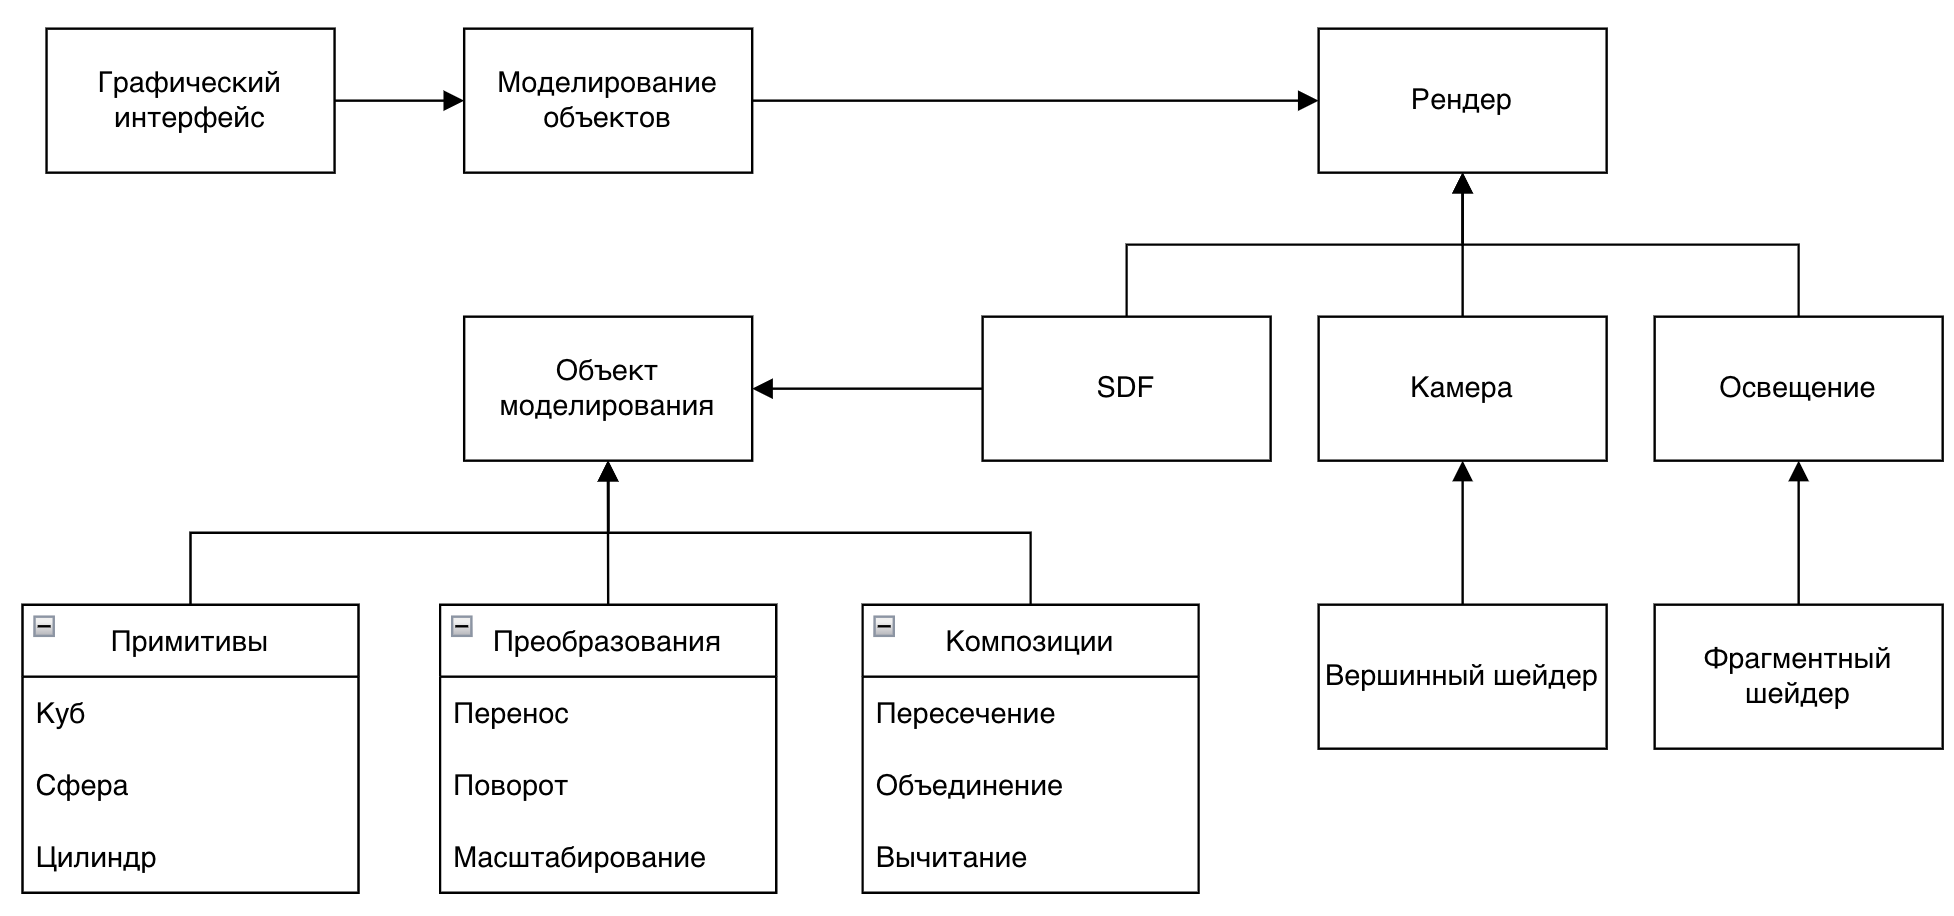
\includegraphics[width=160mm]{img/app.png}
	\caption{Схема приложения}
	\label{fig:app}
\end{figure}

На  данной  схеме  представлена  функциональная  структура  приложения.
Используя  графический  интерфейс,  пользователь  сможет  задать  примитивы, 
положение  камеры,  а  также  используемые  операции  композиции.
Этап моделирования  объектов  представлен  на  рисунке  \ref{fig:modeling} (ниже).
После  него  следует рендер  итогового  изображения  с  использованием  камеры  и  освещения, полученных благодаря вершинному и фрагментному шейдерам.

\begin{figure}[h]
	\centering
	\captionsetup{justification=centering}
	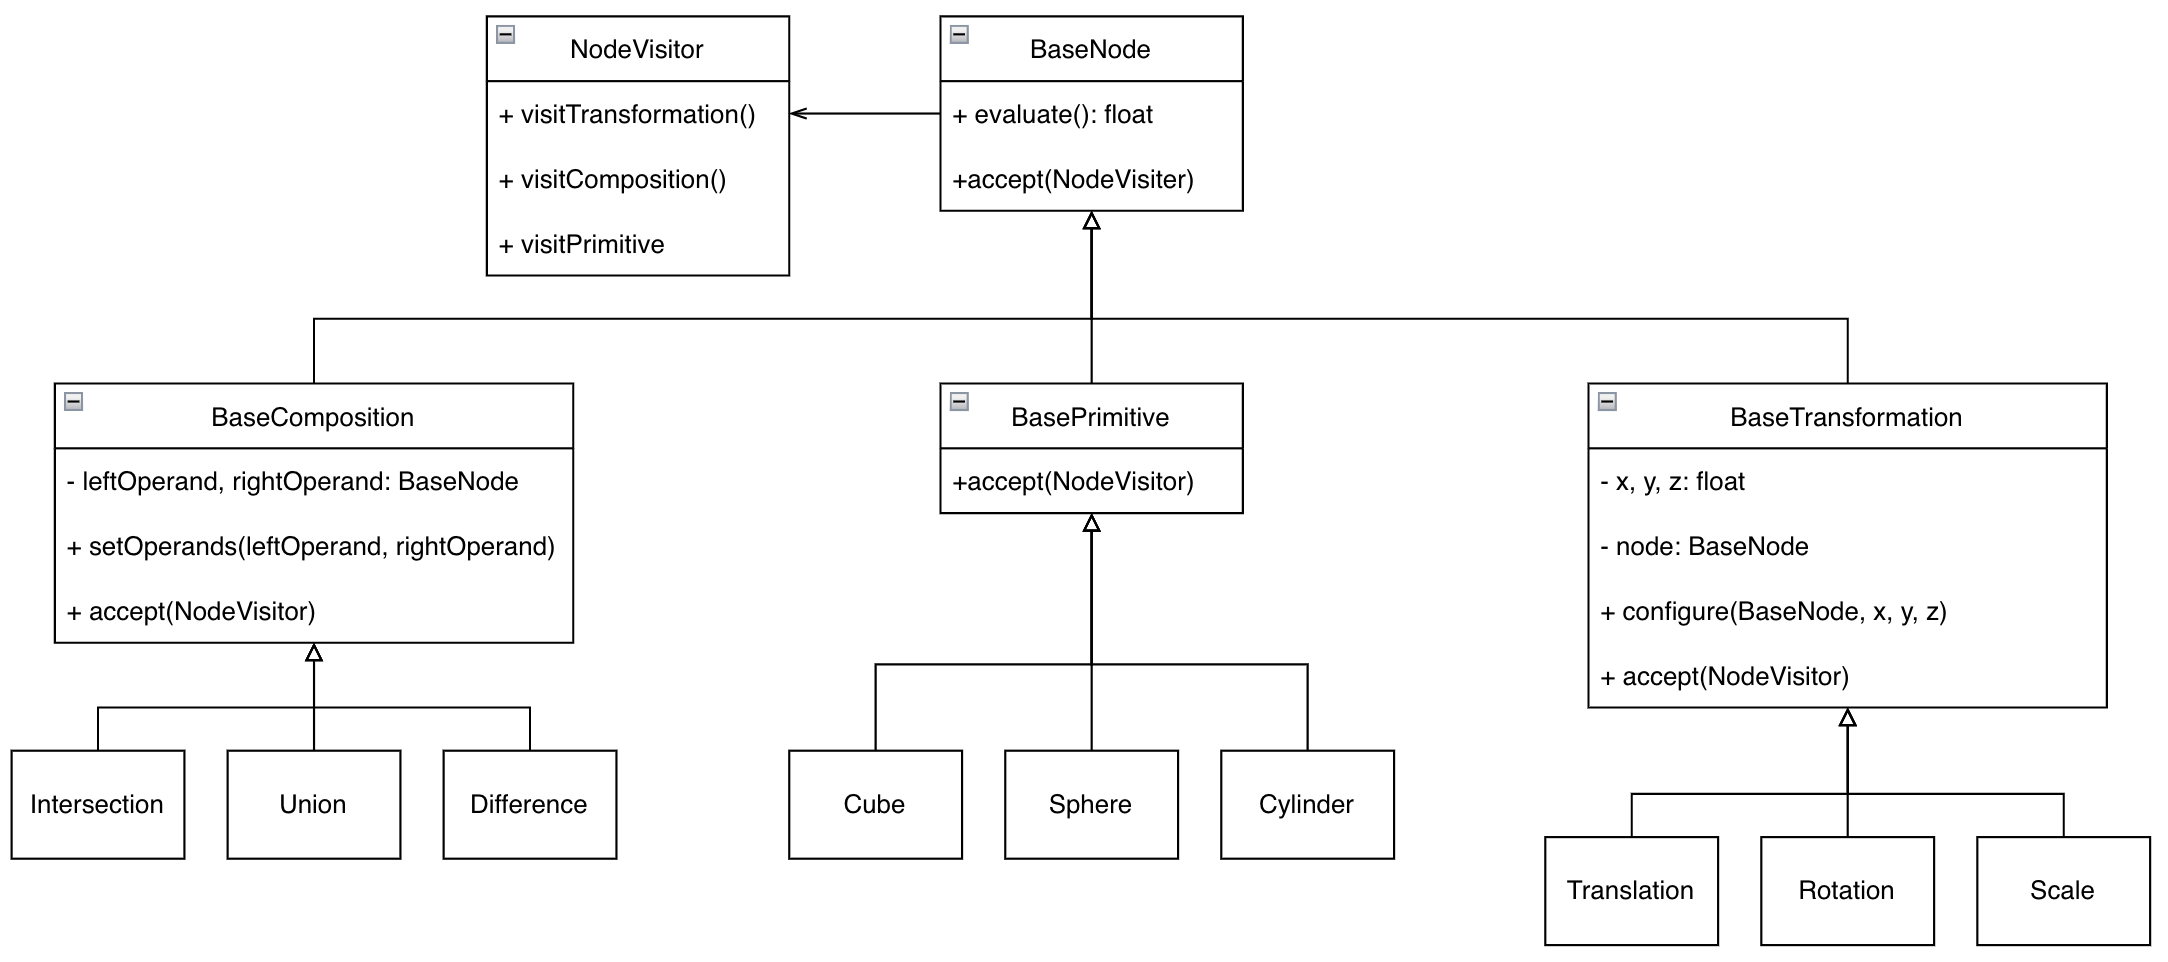
\includegraphics[width=160mm]{img/modeling.png}
	\caption{Диаграмма классов этапа моделирования объектов}
	\label{fig:modeling}
\end{figure}
\clearpage

Поскольку  в  технологии  конструктивной  блочной  геометрии 
используется дерево построений, то в приложении данное дерево представлено 
как двоичное дерево, элементами которого являются объекты класса \textit{BaseNode}, которыми могут быть элементы трансформации, композиции или примитивы --- соответственно, классы \textit{BaseTransformation}, \textit{BaseComposition} и \textit{BasePrimitive}.

Класс  \textit{BaseTransformation} используется  для  преобразования  объекта 
модели  и  содержит  в  себе  необходимые  для  выполнения  операции 
(перемещения, поворота или масштабирования) координаты.
У него есть метод \textit{configure}, который производит настройку экземпляра класса в соответствии с переданным объектом.

Класс  \textit{BaseComposition} используется  для  выполнения  операций композиции (пересечения, объединения и вычитания).
Он представляет собой дерево (построений), результатом обхода которого является итоговая модель.

Класс  \textit{BasePrimitive}  предназначен  для  создания  объектов  модели, 
построение и обработка которых будет осуществляться.

Также  имеется  класс  \textit{NodeVisitor},  реализующий  паттерн  поведения 
«Посетитель», который необходим для добавления нового функционала классам.
Применение данного паттерна помогает абстрагироваться от реализации класса 
\textit{BaseNode} и  предоставить  обход  узлов  дерева  посетителю,  который  будет обходить  узлы  при  помощи  методов  \textit{visitTransformation}, \textit{visitComposition} и \newline \textit{visitPrimitive}.

\subsection*{Вывод}

В данном разделе были рассмотрены методы и алгоритмы, необходимые 
для понимания и создания приложения, а также приведены схема приложения и 
диаграмма классов для этапа моделирования объектов.
\pagebreak